\documentclass[twoside]{book}

% Packages required by doxygen
\usepackage{fixltx2e}
\usepackage{calc}
\usepackage{doxygen}
\usepackage[export]{adjustbox} % also loads graphicx
\usepackage{graphicx}
\usepackage[utf8]{inputenc}
\usepackage{makeidx}
\usepackage{multicol}
\usepackage{multirow}
\PassOptionsToPackage{warn}{textcomp}
\usepackage{textcomp}
\usepackage[nointegrals]{wasysym}
\usepackage[table]{xcolor}

% Font selection
\usepackage[T1]{fontenc}
\usepackage[scaled=.90]{helvet}
\usepackage{courier}
\usepackage{amssymb}
\usepackage{sectsty}
\renewcommand{\familydefault}{\sfdefault}
\allsectionsfont{%
  \fontseries{bc}\selectfont%
  \color{darkgray}%
}
\renewcommand{\DoxyLabelFont}{%
  \fontseries{bc}\selectfont%
  \color{darkgray}%
}
\newcommand{\+}{\discretionary{\mbox{\scriptsize$\hookleftarrow$}}{}{}}

% Page & text layout
\usepackage{geometry}
\geometry{%
  a4paper,%
  top=2.5cm,%
  bottom=2.5cm,%
  left=2.5cm,%
  right=2.5cm%
}
\tolerance=750
\hfuzz=15pt
\hbadness=750
\setlength{\emergencystretch}{15pt}
\setlength{\parindent}{0cm}
\setlength{\parskip}{3ex plus 2ex minus 2ex}
\makeatletter
\renewcommand{\paragraph}{%
  \@startsection{paragraph}{4}{0ex}{-1.0ex}{1.0ex}{%
    \normalfont\normalsize\bfseries\SS@parafont%
  }%
}
\renewcommand{\subparagraph}{%
  \@startsection{subparagraph}{5}{0ex}{-1.0ex}{1.0ex}{%
    \normalfont\normalsize\bfseries\SS@subparafont%
  }%
}
\makeatother

% Headers & footers
\usepackage{fancyhdr}
\pagestyle{fancyplain}
\fancyhead[LE]{\fancyplain{}{\bfseries\thepage}}
\fancyhead[CE]{\fancyplain{}{}}
\fancyhead[RE]{\fancyplain{}{\bfseries\leftmark}}
\fancyhead[LO]{\fancyplain{}{\bfseries\rightmark}}
\fancyhead[CO]{\fancyplain{}{}}
\fancyhead[RO]{\fancyplain{}{\bfseries\thepage}}
\fancyfoot[LE]{\fancyplain{}{}}
\fancyfoot[CE]{\fancyplain{}{}}
\fancyfoot[RE]{\fancyplain{}{\bfseries\scriptsize Generated by Doxygen }}
\fancyfoot[LO]{\fancyplain{}{\bfseries\scriptsize Generated by Doxygen }}
\fancyfoot[CO]{\fancyplain{}{}}
\fancyfoot[RO]{\fancyplain{}{}}
\renewcommand{\footrulewidth}{0.4pt}
\renewcommand{\chaptermark}[1]{%
  \markboth{#1}{}%
}
\renewcommand{\sectionmark}[1]{%
  \markright{\thesection\ #1}%
}

% Indices & bibliography
\usepackage{natbib}
\usepackage[titles]{tocloft}
\setcounter{tocdepth}{3}
\setcounter{secnumdepth}{5}
\makeindex

% Hyperlinks (required, but should be loaded last)
\usepackage{ifpdf}
\ifpdf
  \usepackage[pdftex,pagebackref=true]{hyperref}
\else
  \usepackage[ps2pdf,pagebackref=true]{hyperref}
\fi
\hypersetup{%
  colorlinks=true,%
  linkcolor=blue,%
  citecolor=blue,%
  unicode%
}

% Custom commands
\newcommand{\clearemptydoublepage}{%
  \newpage{\pagestyle{empty}\cleardoublepage}%
}

\usepackage{caption}
\captionsetup{labelsep=space,justification=centering,font={bf},singlelinecheck=off,skip=4pt,position=top}

%===== C O N T E N T S =====

\begin{document}

% Titlepage & ToC
\hypersetup{pageanchor=false,
             bookmarksnumbered=true,
             pdfencoding=unicode
            }
\pagenumbering{roman}
\begin{titlepage}
\vspace*{7cm}
\begin{center}%
{\Large S\+F\+GF }\\
\vspace*{1cm}
{\large Generated by Doxygen 1.8.11}\\
\end{center}
\end{titlepage}
\clearemptydoublepage
\tableofcontents
\clearemptydoublepage
\pagenumbering{arabic}
\hypersetup{pageanchor=true}

%--- Begin generated contents ---
\chapter{S\+F\+GF}
\label{index}\hypertarget{index}{}\hypertarget{index_sfgf}{}\section{sfgf}\label{index_sfgf}
Simple and Fast Game Framework. Based on… yes, S\+F\+M\+L!\hypertarget{index_motivation}{}\section{motivation}\label{index_motivation}
I really wanted to have some more complex game–related A\+PI on top on S\+F\+ML, couldn\textquotesingle{}t find anything on internet and… well, what could I do excluding writing it myself?\hypertarget{index_Aim}{}\section{Aim}\label{index_Aim}

\begin{DoxyItemize}
\item Rather high level, no need to understand Open\+GL.
\item Polygon–based collision detection.
\item Children–\+Parent node chierarchy.
\item Some set of basic classes.
\item Easly extendible.
\item Header–only.
\end{DoxyItemize}\hypertarget{index_Collaboration}{}\section{Collaboration}\label{index_Collaboration}
I\textquotesingle{}m open to proposals, if you want to add something from yourself post a feature request in \textquotesingle{}Issues\textquotesingle{} tab or e–mail me (\href{mailto:koczurekk@gmail.com}{\tt koczurekk@gmail.\+com}). 
\chapter{Namespace Index}
\section{Namespace List}
Here is a list of all documented namespaces with brief descriptions\+:\begin{DoxyCompactList}
\item\contentsline{section}{\hyperlink{namespacesfgf}{sfgf} \\*Contains all S\+F\+GF classes }{\pageref{namespacesfgf}}{}
\end{DoxyCompactList}

\chapter{Hierarchical Index}
\section{Class Hierarchy}
This inheritance list is sorted roughly, but not completely, alphabetically\+:\begin{DoxyCompactList}
\item \contentsline{section}{sfgf\+:\+:Collider}{\pageref{classsfgf_1_1Collider}}{}
\item \contentsline{section}{sfgf\+:\+:Copy\+Lock}{\pageref{classsfgf_1_1CopyLock}}{}
\item Drawable\begin{DoxyCompactList}
\item \contentsline{section}{sfgf\+:\+:Polygon}{\pageref{classsfgf_1_1Polygon}}{}
\begin{DoxyCompactList}
\item \contentsline{section}{sfgf\+:\+:Plane}{\pageref{classsfgf_1_1Plane}}{}
\end{DoxyCompactList}
\end{DoxyCompactList}
\item \contentsline{section}{sfgf\+:\+:Object\+Pack}{\pageref{classsfgf_1_1ObjectPack}}{}
\item Transformable\begin{DoxyCompactList}
\item \contentsline{section}{sfgf\+:\+:Game\+Object}{\pageref{classsfgf_1_1GameObject}}{}
\begin{DoxyCompactList}
\item \contentsline{section}{sfgf\+:\+:Polygon}{\pageref{classsfgf_1_1Polygon}}{}
\end{DoxyCompactList}
\end{DoxyCompactList}
\end{DoxyCompactList}

\chapter{Class Index}
\section{Class List}
Here are the classes, structs, unions and interfaces with brief descriptions\+:\begin{DoxyCompactList}
\item\contentsline{section}{\hyperlink{classsfgf_1_1Collider}{sfgf\+::\+Collider} \\*Handles collisions }{\pageref{classsfgf_1_1Collider}}{}
\item\contentsline{section}{\hyperlink{classsfgf_1_1CopyLock}{sfgf\+::\+Copy\+Lock} }{\pageref{classsfgf_1_1CopyLock}}{}
\item\contentsline{section}{\hyperlink{classsfgf_1_1GameObject}{sfgf\+::\+Game\+Object} }{\pageref{classsfgf_1_1GameObject}}{}
\item\contentsline{section}{\hyperlink{classsfgf_1_1ObjectPack}{sfgf\+::\+Object\+Pack} }{\pageref{classsfgf_1_1ObjectPack}}{}
\item\contentsline{section}{\hyperlink{classsfgf_1_1Plane}{sfgf\+::\+Plane} }{\pageref{classsfgf_1_1Plane}}{}
\item\contentsline{section}{\hyperlink{classsfgf_1_1Polygon}{sfgf\+::\+Polygon} }{\pageref{classsfgf_1_1Polygon}}{}
\end{DoxyCompactList}

\chapter{File Index}
\section{File List}
Here is a list of all documented files with brief descriptions\+:\begin{DoxyCompactList}
\item\contentsline{section}{S\+F\+G\+F/\hyperlink{Collider_8hpp}{Collider.\+hpp} \\*Collider class implementation }{\pageref{Collider_8hpp}}{}
\item\contentsline{section}{S\+F\+G\+F/{\bfseries Copy\+Lock.\+hpp} }{\pageref{CopyLock_8hpp}}{}
\item\contentsline{section}{S\+F\+G\+F/{\bfseries Game\+Object.\+hpp} }{\pageref{GameObject_8hpp}}{}
\item\contentsline{section}{S\+F\+G\+F/{\bfseries Object\+Pack.\+hpp} }{\pageref{ObjectPack_8hpp}}{}
\item\contentsline{section}{S\+F\+G\+F/{\bfseries Plane.\+hpp} }{\pageref{Plane_8hpp}}{}
\item\contentsline{section}{S\+F\+G\+F/{\bfseries Polygon.\+hpp} }{\pageref{Polygon_8hpp}}{}
\end{DoxyCompactList}

\chapter{Namespace Documentation}
\hypertarget{namespacesfgf}{}\section{sfgf Namespace Reference}
\label{namespacesfgf}\index{sfgf@{sfgf}}


Contains all S\+F\+GF classes.  


\subsection*{Classes}
\begin{DoxyCompactItemize}
\item 
class \hyperlink{classsfgf_1_1Collider}{Collider}
\begin{DoxyCompactList}\small\item\em Handles collisions. \end{DoxyCompactList}\item 
class \hyperlink{classsfgf_1_1CopyLock}{Copy\+Lock}
\item 
class \hyperlink{classsfgf_1_1GameObject}{Game\+Object}
\item 
class \hyperlink{classsfgf_1_1ObjectPack}{Object\+Pack}
\item 
class \hyperlink{classsfgf_1_1Plane}{Plane}
\item 
class \hyperlink{classsfgf_1_1Polygon}{Polygon}
\end{DoxyCompactItemize}


\subsection{Detailed Description}
Contains all S\+F\+GF classes. 
\chapter{Class Documentation}
\hypertarget{classsfgf_1_1Collider}{}\section{sfgf\+:\+:Collider Class Reference}
\label{classsfgf_1_1Collider}\index{sfgf\+::\+Collider@{sfgf\+::\+Collider}}


Handles collisions.  




{\ttfamily \#include $<$Collider.\+hpp$>$}

\subsection*{Public Member Functions}
\begin{DoxyCompactItemize}
\item 
void \hyperlink{classsfgf_1_1Collider_ab76aa2334b97723309dec9c06f13e5aa}{apply\+Transform} (const sf\+::\+Transform \&t)
\begin{DoxyCompactList}\small\item\em Applies transform. \end{DoxyCompactList}\item 
void \hyperlink{classsfgf_1_1Collider_ac7ada2ab00581dccb5d4590d0ec80d57}{push\+Back} (sf\+::\+Vector2f pt)
\begin{DoxyCompactList}\small\item\em Adds point to internal array. \end{DoxyCompactList}\item 
void \hyperlink{classsfgf_1_1Collider_a4db86f18fef1c67dfa2523f106096fc8}{clear} ()
\begin{DoxyCompactList}\small\item\em Clears points. \end{DoxyCompactList}\item 
sf\+::\+Float\+Rect \hyperlink{classsfgf_1_1Collider_a7625649032857e18d7b27bd7bed18c24}{get\+Global\+Bounds} () const 
\begin{DoxyCompactList}\small\item\em Returns global bounds. \end{DoxyCompactList}\item 
bool \hyperlink{classsfgf_1_1Collider_ad6a628c00cfd66ccb06792c91305007e}{intersects} (const \hyperlink{classsfgf_1_1Collider}{Collider} \&poly) const 
\begin{DoxyCompactList}\small\item\em Check for intersection. \end{DoxyCompactList}\item 
bool \hyperlink{classsfgf_1_1Collider_af193ced12d857c8cec6f604ae4d9c905}{contains} (sf\+::\+Vector2f point) const 
\begin{DoxyCompactList}\small\item\em Check if point is inside of collider. \end{DoxyCompactList}\item 
bool \hyperlink{classsfgf_1_1Collider_a51b98794c87237d2cbf4cf3fdbfd2c62}{collides} (const \hyperlink{classsfgf_1_1Collider}{Collider} \&poly) const 
\begin{DoxyCompactList}\small\item\em Check if two colliders collide. \end{DoxyCompactList}\end{DoxyCompactItemize}
\subsection*{Static Public Member Functions}
\begin{DoxyCompactItemize}
\item 
static \hyperlink{classsfgf_1_1Collider}{Collider} \hyperlink{classsfgf_1_1Collider_a22251044e824c236f250689c4023c992}{circle} (float radius, size\+\_\+t cnt=128)
\begin{DoxyCompactList}\small\item\em Returns collider in shape of circle. \end{DoxyCompactList}\item 
static \hyperlink{classsfgf_1_1Collider}{Collider} \hyperlink{classsfgf_1_1Collider_aaf00da4b750ec490048de061c98d8ad0}{rectangle} (sf\+::\+Vector2f size)
\begin{DoxyCompactList}\small\item\em Returns collider in shape of rectangle. \end{DoxyCompactList}\item 
static bool \hyperlink{classsfgf_1_1Collider_a2e1731b6dfd829261e763154e5a27904}{line\+Intersection} (sf\+::\+Vector2f p1, sf\+::\+Vector2f q1, sf\+::\+Vector2f p2, sf\+::\+Vector2f q2)
\begin{DoxyCompactList}\small\item\em Check two lines for intersection. \end{DoxyCompactList}\end{DoxyCompactItemize}


\subsection{Detailed Description}
Handles collisions. 

Contains basic set of points which can be later transformed to represent bounds of an object. Also supports global\+Bounds to make collision detection more efficient. ~\newline
 Sample code\+: 
\begin{DoxyCode}
\textcolor{keyword}{auto} \hyperlink{classsfgf_1_1Collider_a22251044e824c236f250689c4023c992}{circle} = \hyperlink{classsfgf_1_1Collider_a22251044e824c236f250689c4023c992}{sfgf::Collider::circle}(5); \textcolor{comment}{// Make circle, r = 5}
\textcolor{keyword}{auto} rect = \hyperlink{classsfgf_1_1Collider_aaf00da4b750ec490048de061c98d8ad0}{sfgf::Collider::rectangle}(\{10, 10\}); \textcolor{comment}{// Make rectangle (10, 10)}

\textcolor{keyword}{auto} t = sf::Transform().translate(\{9, 0\}); \textcolor{comment}{// Make transform translating by 9 to the right}
\hyperlink{classsfgf_1_1Collider_a22251044e824c236f250689c4023c992}{circle}.\hyperlink{classsfgf_1_1Collider_ab76aa2334b97723309dec9c06f13e5aa}{applyTransform}(t); \textcolor{comment}{// Apply that transform to circle}

std::cout << std::boolalpha << \hyperlink{classsfgf_1_1Collider_a22251044e824c236f250689c4023c992}{circle}.\hyperlink{classsfgf_1_1Collider_a51b98794c87237d2cbf4cf3fdbfd2c62}{collides}(rect) << std::endl; \textcolor{comment}{//True}
\hyperlink{classsfgf_1_1Collider_a22251044e824c236f250689c4023c992}{circle}.\hyperlink{classsfgf_1_1Collider_ab76aa2334b97723309dec9c06f13e5aa}{applyTransform}(t); \textcolor{comment}{// Apply transform again}
std::cout << std::boolalpha << \hyperlink{classsfgf_1_1Collider_a22251044e824c236f250689c4023c992}{circle}.\hyperlink{classsfgf_1_1Collider_a51b98794c87237d2cbf4cf3fdbfd2c62}{collides}(rect) << std::endl; \textcolor{comment}{//False}
\end{DoxyCode}
 

\subsection{Member Function Documentation}
\index{sfgf\+::\+Collider@{sfgf\+::\+Collider}!apply\+Transform@{apply\+Transform}}
\index{apply\+Transform@{apply\+Transform}!sfgf\+::\+Collider@{sfgf\+::\+Collider}}
\subsubsection[{\texorpdfstring{apply\+Transform(const sf\+::\+Transform \&t)}{applyTransform(const sf::Transform &t)}}]{\setlength{\rightskip}{0pt plus 5cm}void sfgf\+::\+Collider\+::apply\+Transform (
\begin{DoxyParamCaption}
\item[{const sf\+::\+Transform \&}]{t}
\end{DoxyParamCaption}
)}\hypertarget{classsfgf_1_1Collider_ab76aa2334b97723309dec9c06f13e5aa}{}\label{classsfgf_1_1Collider_ab76aa2334b97723309dec9c06f13e5aa}


Applies transform. 


\begin{DoxyParams}[1]{Parameters}
\mbox{\tt in}  & {\em t} & – transform to use\\
\hline
\end{DoxyParams}
Used to adjust position/rotation/scale of collider to actual object.~\newline
 Sample code\+: 
\begin{DoxyCode}
this->collider.applyTransform(this->polygon.getTransform());
\end{DoxyCode}
 \index{sfgf\+::\+Collider@{sfgf\+::\+Collider}!circle@{circle}}
\index{circle@{circle}!sfgf\+::\+Collider@{sfgf\+::\+Collider}}
\subsubsection[{\texorpdfstring{circle(float radius, size\+\_\+t cnt=128)}{circle(float radius, size_t cnt=128)}}]{\setlength{\rightskip}{0pt plus 5cm}{\bf Collider} sfgf\+::\+Collider\+::circle (
\begin{DoxyParamCaption}
\item[{float}]{radius, }
\item[{size\+\_\+t}]{cnt = {\ttfamily 128}}
\end{DoxyParamCaption}
)\hspace{0.3cm}{\ttfamily [static]}}\hypertarget{classsfgf_1_1Collider_a22251044e824c236f250689c4023c992}{}\label{classsfgf_1_1Collider_a22251044e824c236f250689c4023c992}


Returns collider in shape of circle. 


\begin{DoxyParams}[1]{Parameters}
\mbox{\tt in}  & {\em radius} & – radius of circle \\
\hline
\mbox{\tt in}  & {\em cnt} & – count of points to make\\
\hline
\end{DoxyParams}
\begin{DoxyReturn}{Returns}
new collider
\end{DoxyReturn}

\begin{DoxyCode}
somePolygon.setSampleCollider(\hyperlink{classsfgf_1_1Collider_a22251044e824c236f250689c4023c992}{sfgf::Collider::circle}(7));
\end{DoxyCode}
 \index{sfgf\+::\+Collider@{sfgf\+::\+Collider}!clear@{clear}}
\index{clear@{clear}!sfgf\+::\+Collider@{sfgf\+::\+Collider}}
\subsubsection[{\texorpdfstring{clear()}{clear()}}]{\setlength{\rightskip}{0pt plus 5cm}void sfgf\+::\+Collider\+::clear (
\begin{DoxyParamCaption}
{}
\end{DoxyParamCaption}
)}\hypertarget{classsfgf_1_1Collider_a4db86f18fef1c67dfa2523f106096fc8}{}\label{classsfgf_1_1Collider_a4db86f18fef1c67dfa2523f106096fc8}


Clears points. 

Simply clears internal array (std\+::vector), empty collider never detects any collision. \index{sfgf\+::\+Collider@{sfgf\+::\+Collider}!collides@{collides}}
\index{collides@{collides}!sfgf\+::\+Collider@{sfgf\+::\+Collider}}
\subsubsection[{\texorpdfstring{collides(const Collider \&poly) const }{collides(const Collider &poly) const }}]{\setlength{\rightskip}{0pt plus 5cm}bool sfgf\+::\+Collider\+::collides (
\begin{DoxyParamCaption}
\item[{const {\bf Collider} \&}]{poly}
\end{DoxyParamCaption}
) const}\hypertarget{classsfgf_1_1Collider_a51b98794c87237d2cbf4cf3fdbfd2c62}{}\label{classsfgf_1_1Collider_a51b98794c87237d2cbf4cf3fdbfd2c62}


Check if two colliders collide. 


\begin{DoxyParams}[1]{Parameters}
\mbox{\tt in}  & {\em poly} & – collider to check against\\
\hline
\end{DoxyParams}
Tests whether colliders collide or not. They do, if any of theirs side intersect or if no point of one collider is outside of another.

\begin{DoxyReturn}{Returns}
True if they collide, False otherwise. 
\end{DoxyReturn}
\index{sfgf\+::\+Collider@{sfgf\+::\+Collider}!contains@{contains}}
\index{contains@{contains}!sfgf\+::\+Collider@{sfgf\+::\+Collider}}
\subsubsection[{\texorpdfstring{contains(sf\+::\+Vector2f point) const }{contains(sf::Vector2f point) const }}]{\setlength{\rightskip}{0pt plus 5cm}bool sfgf\+::\+Collider\+::contains (
\begin{DoxyParamCaption}
\item[{sf\+::\+Vector2f}]{point}
\end{DoxyParamCaption}
) const}\hypertarget{classsfgf_1_1Collider_af193ced12d857c8cec6f604ae4d9c905}{}\label{classsfgf_1_1Collider_af193ced12d857c8cec6f604ae4d9c905}


Check if point is inside of collider. 


\begin{DoxyParams}[1]{Parameters}
\mbox{\tt in}  & {\em point} & – point to check\\
\hline
\end{DoxyParams}
Tests if given point is inside of ($\ast$this).

\begin{DoxyReturn}{Returns}
True if point is in collider, false otherwise 
\end{DoxyReturn}
\index{sfgf\+::\+Collider@{sfgf\+::\+Collider}!get\+Global\+Bounds@{get\+Global\+Bounds}}
\index{get\+Global\+Bounds@{get\+Global\+Bounds}!sfgf\+::\+Collider@{sfgf\+::\+Collider}}
\subsubsection[{\texorpdfstring{get\+Global\+Bounds() const }{getGlobalBounds() const }}]{\setlength{\rightskip}{0pt plus 5cm}sf\+::\+Float\+Rect sfgf\+::\+Collider\+::get\+Global\+Bounds (
\begin{DoxyParamCaption}
{}
\end{DoxyParamCaption}
) const\hspace{0.3cm}{\ttfamily [inline]}}\hypertarget{classsfgf_1_1Collider_a7625649032857e18d7b27bd7bed18c24}{}\label{classsfgf_1_1Collider_a7625649032857e18d7b27bd7bed18c24}


Returns global bounds. 

Get the global bounding rectangle of the entity. ~\newline
 The returned rectangle is in global coordinates, which means that it takes in account the transformations (translation, rotation, scale, …) that are applied to the entity. In other words, this function returns the bounds of the collider in the global 2D world\textquotesingle{}s coordinate system.

\begin{DoxyReturn}{Returns}
Global bounding rectangle of the entity 
\end{DoxyReturn}
\index{sfgf\+::\+Collider@{sfgf\+::\+Collider}!intersects@{intersects}}
\index{intersects@{intersects}!sfgf\+::\+Collider@{sfgf\+::\+Collider}}
\subsubsection[{\texorpdfstring{intersects(const Collider \&poly) const }{intersects(const Collider &poly) const }}]{\setlength{\rightskip}{0pt plus 5cm}bool sfgf\+::\+Collider\+::intersects (
\begin{DoxyParamCaption}
\item[{const {\bf Collider} \&}]{poly}
\end{DoxyParamCaption}
) const}\hypertarget{classsfgf_1_1Collider_ad6a628c00cfd66ccb06792c91305007e}{}\label{classsfgf_1_1Collider_ad6a628c00cfd66ccb06792c91305007e}


Check for intersection. 


\begin{DoxyParams}[1]{Parameters}
\mbox{\tt in}  & {\em poly} & – collider to check\\
\hline
\end{DoxyParams}
Tests if any side of ($\ast$this) intersects with any side of poly.

\begin{DoxyReturn}{Returns}
True if colliders intersect, False otherwise 
\end{DoxyReturn}
\index{sfgf\+::\+Collider@{sfgf\+::\+Collider}!line\+Intersection@{line\+Intersection}}
\index{line\+Intersection@{line\+Intersection}!sfgf\+::\+Collider@{sfgf\+::\+Collider}}
\subsubsection[{\texorpdfstring{line\+Intersection(sf\+::\+Vector2f p1, sf\+::\+Vector2f q1, sf\+::\+Vector2f p2, sf\+::\+Vector2f q2)}{lineIntersection(sf::Vector2f p1, sf::Vector2f q1, sf::Vector2f p2, sf::Vector2f q2)}}]{\setlength{\rightskip}{0pt plus 5cm}bool sfgf\+::\+Collider\+::line\+Intersection (
\begin{DoxyParamCaption}
\item[{sf\+::\+Vector2f}]{p1, }
\item[{sf\+::\+Vector2f}]{q1, }
\item[{sf\+::\+Vector2f}]{p2, }
\item[{sf\+::\+Vector2f}]{q2}
\end{DoxyParamCaption}
)\hspace{0.3cm}{\ttfamily [static]}}\hypertarget{classsfgf_1_1Collider_a2e1731b6dfd829261e763154e5a27904}{}\label{classsfgf_1_1Collider_a2e1731b6dfd829261e763154e5a27904}


Check two lines for intersection. 


\begin{DoxyParams}[1]{Parameters}
\mbox{\tt in}  & {\em p1} & – beginning of line I \\
\hline
\mbox{\tt in}  & {\em q1} & – end of line I \\
\hline
\mbox{\tt in}  & {\em p2} & – beginning of line II \\
\hline
\mbox{\tt in}  & {\em q2} & – end of line II\\
\hline
\end{DoxyParams}
\begin{DoxyReturn}{Returns}
True if lines intersect, False otherwise
\end{DoxyReturn}

\begin{DoxyCode}
std::cout << std::boolapha << \hyperlink{classsfgf_1_1Collider_a2e1731b6dfd829261e763154e5a27904}{sfgf::Collider::lineIntersection}(\{0, 0\}, \{50,
       20\}, \{25, 0\}, \{25 50\}) << std::endl;
\end{DoxyCode}
 \index{sfgf\+::\+Collider@{sfgf\+::\+Collider}!push\+Back@{push\+Back}}
\index{push\+Back@{push\+Back}!sfgf\+::\+Collider@{sfgf\+::\+Collider}}
\subsubsection[{\texorpdfstring{push\+Back(sf\+::\+Vector2f pt)}{pushBack(sf::Vector2f pt)}}]{\setlength{\rightskip}{0pt plus 5cm}void sfgf\+::\+Collider\+::push\+Back (
\begin{DoxyParamCaption}
\item[{sf\+::\+Vector2f}]{pt}
\end{DoxyParamCaption}
)}\hypertarget{classsfgf_1_1Collider_ac7ada2ab00581dccb5d4590d0ec80d57}{}\label{classsfgf_1_1Collider_ac7ada2ab00581dccb5d4590d0ec80d57}


Adds point to internal array. 


\begin{DoxyParams}[1]{Parameters}
\mbox{\tt in}  & {\em pt} & – coordinates in local system\\
\hline
\end{DoxyParams}
Can be used to create collider in non–standard shape, aka custom polygon. ~\newline
 Sample code\+: 
\begin{DoxyCode}
\textcolor{keywordflow}{while}(inputFile >> x >> y) \{
    collider.pushBack(\{x, y\});
\}
\end{DoxyCode}
 \index{sfgf\+::\+Collider@{sfgf\+::\+Collider}!rectangle@{rectangle}}
\index{rectangle@{rectangle}!sfgf\+::\+Collider@{sfgf\+::\+Collider}}
\subsubsection[{\texorpdfstring{rectangle(sf\+::\+Vector2f size)}{rectangle(sf::Vector2f size)}}]{\setlength{\rightskip}{0pt plus 5cm}{\bf Collider} sfgf\+::\+Collider\+::rectangle (
\begin{DoxyParamCaption}
\item[{sf\+::\+Vector2f}]{size}
\end{DoxyParamCaption}
)\hspace{0.3cm}{\ttfamily [static]}}\hypertarget{classsfgf_1_1Collider_aaf00da4b750ec490048de061c98d8ad0}{}\label{classsfgf_1_1Collider_aaf00da4b750ec490048de061c98d8ad0}


Returns collider in shape of rectangle. 


\begin{DoxyParams}[1]{Parameters}
\mbox{\tt in}  & {\em size} & – dimensions of rectangle\\
\hline
\end{DoxyParams}
\begin{DoxyReturn}{Returns}
new collider
\end{DoxyReturn}

\begin{DoxyCode}
somePolygon.setSampleCollider(\hyperlink{classsfgf_1_1Collider_aaf00da4b750ec490048de061c98d8ad0}{sfgf::Collider::rectangle}(\{20, 10\}));
\end{DoxyCode}
 

The documentation for this class was generated from the following file\+:\begin{DoxyCompactItemize}
\item 
S\+F\+G\+F/\hyperlink{Collider_8hpp}{Collider.\+hpp}\end{DoxyCompactItemize}

\hypertarget{classsfgf_1_1CopyLock}{}\section{sfgf\+:\+:Copy\+Lock Class Reference}
\label{classsfgf_1_1CopyLock}\index{sfgf\+::\+Copy\+Lock@{sfgf\+::\+Copy\+Lock}}


The documentation for this class was generated from the following file\+:\begin{DoxyCompactItemize}
\item 
S\+F\+G\+F/Copy\+Lock.\+hpp\end{DoxyCompactItemize}

\hypertarget{classsfgf_1_1GameObject}{}\section{sfgf\+:\+:Game\+Object Class Reference}
\label{classsfgf_1_1GameObject}\index{sfgf\+::\+Game\+Object@{sfgf\+::\+Game\+Object}}


Inheritance diagram for sfgf\+:\+:Game\+Object\+:\nopagebreak
\begin{figure}[H]
\begin{center}
\leavevmode
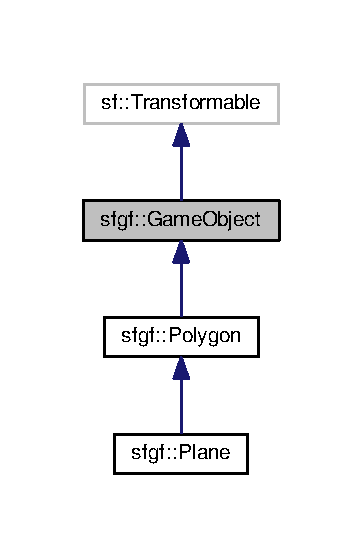
\includegraphics[width=174pt]{classsfgf_1_1GameObject__inherit__graph}
\end{center}
\end{figure}
\subsection*{Public Member Functions}
\begin{DoxyCompactItemize}
\item 
virtual void {\bfseries update} (sf\+::\+Time)\hypertarget{classsfgf_1_1GameObject_a0bf26d2cfdf041d3fe487cd3f44a48d9}{}\label{classsfgf_1_1GameObject_a0bf26d2cfdf041d3fe487cd3f44a48d9}

\item 
void {\bfseries set\+Parent} (const \hyperlink{classsfgf_1_1GameObject}{Game\+Object} \&parent)\hypertarget{classsfgf_1_1GameObject_ad7ca320499bed4ea5acd0cfadbd4031a}{}\label{classsfgf_1_1GameObject_ad7ca320499bed4ea5acd0cfadbd4031a}

\item 
const \hyperlink{classsfgf_1_1GameObject}{Game\+Object} \& {\bfseries get\+Parent} () const \hypertarget{classsfgf_1_1GameObject_a4c96ad96e5aa58d93f41b4896f95ff12}{}\label{classsfgf_1_1GameObject_a4c96ad96e5aa58d93f41b4896f95ff12}

\item 
sf\+::\+Transform {\bfseries get\+Transform} () const \hypertarget{classsfgf_1_1GameObject_a09b30b373b460ef9ad7b07faeb274324}{}\label{classsfgf_1_1GameObject_a09b30b373b460ef9ad7b07faeb274324}

\end{DoxyCompactItemize}


The documentation for this class was generated from the following file\+:\begin{DoxyCompactItemize}
\item 
S\+F\+G\+F/Game\+Object.\+hpp\end{DoxyCompactItemize}

\hypertarget{classsfgf_1_1ObjectPack}{}\section{sfgf\+:\+:Object\+Pack Class Reference}
\label{classsfgf_1_1ObjectPack}\index{sfgf\+::\+Object\+Pack@{sfgf\+::\+Object\+Pack}}
\subsection*{Public Member Functions}
\begin{DoxyCompactItemize}
\item 
{\footnotesize template$<$class... args\+\_\+t$>$ }\\{\bfseries Object\+Pack} (args\+\_\+t \&...list)\hypertarget{classsfgf_1_1ObjectPack_ae3b64ca6ce9abb374c7dcab82004f33c}{}\label{classsfgf_1_1ObjectPack_ae3b64ca6ce9abb374c7dcab82004f33c}

\item 
void {\bfseries add} (\hyperlink{classsfgf_1_1GameObject}{Game\+Object} \&obj)\hypertarget{classsfgf_1_1ObjectPack_a811af32e24df6029047ca9ee13e9e048}{}\label{classsfgf_1_1ObjectPack_a811af32e24df6029047ca9ee13e9e048}

\item 
void {\bfseries remove} (\hyperlink{classsfgf_1_1GameObject}{Game\+Object} \&obj)\hypertarget{classsfgf_1_1ObjectPack_ae34a71c478e3878b6b9d2e3e75a209da}{}\label{classsfgf_1_1ObjectPack_ae34a71c478e3878b6b9d2e3e75a209da}

\item 
void {\bfseries update} (sf\+::\+Time t)\hypertarget{classsfgf_1_1ObjectPack_aba9d69c11b84d2e1cd46399b884451bc}{}\label{classsfgf_1_1ObjectPack_aba9d69c11b84d2e1cd46399b884451bc}

\end{DoxyCompactItemize}


The documentation for this class was generated from the following file\+:\begin{DoxyCompactItemize}
\item 
S\+F\+G\+F/Object\+Pack.\+hpp\end{DoxyCompactItemize}

\hypertarget{classsfgf_1_1Plane}{}\section{sfgf\+:\+:Plane Class Reference}
\label{classsfgf_1_1Plane}\index{sfgf\+::\+Plane@{sfgf\+::\+Plane}}


Inheritance diagram for sfgf\+:\+:Plane\+:\nopagebreak
\begin{figure}[H]
\begin{center}
\leavevmode
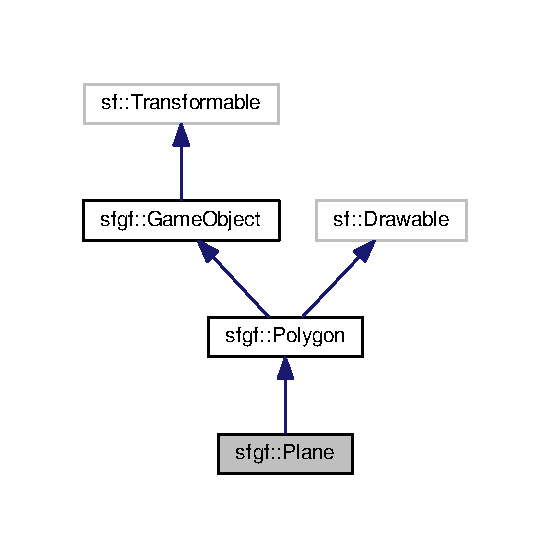
\includegraphics[width=264pt]{classsfgf_1_1Plane__inherit__graph}
\end{center}
\end{figure}
\subsection*{Public Member Functions}
\begin{DoxyCompactItemize}
\item 
void {\bfseries set\+Texture} (const sf\+::\+Texture \&tex)\hypertarget{classsfgf_1_1Plane_a9a99e5944b94b8a7b565072c73c67a1d}{}\label{classsfgf_1_1Plane_a9a99e5944b94b8a7b565072c73c67a1d}

\item 
void {\bfseries set\+Size} (sf\+::\+Vector2f size)\hypertarget{classsfgf_1_1Plane_a70c92e0de46c76339f37efe40a77b939}{}\label{classsfgf_1_1Plane_a70c92e0de46c76339f37efe40a77b939}

\item 
sf\+::\+Vector2f {\bfseries get\+Size} () const \hypertarget{classsfgf_1_1Plane_ab6f328c5d7cfb2902af7498333a019fe}{}\label{classsfgf_1_1Plane_ab6f328c5d7cfb2902af7498333a019fe}

\item 
void {\bfseries self\+Center} ()\hypertarget{classsfgf_1_1Plane_a30b427bbc8be38c99501b91db6b5a4c0}{}\label{classsfgf_1_1Plane_a30b427bbc8be38c99501b91db6b5a4c0}

\end{DoxyCompactItemize}


The documentation for this class was generated from the following file\+:\begin{DoxyCompactItemize}
\item 
S\+F\+G\+F/Plane.\+hpp\end{DoxyCompactItemize}

\hypertarget{classsfgf_1_1Polygon}{}\section{sfgf\+:\+:Polygon Class Reference}
\label{classsfgf_1_1Polygon}\index{sfgf\+::\+Polygon@{sfgf\+::\+Polygon}}


Inheritance diagram for sfgf\+:\+:Polygon\+:\nopagebreak
\begin{figure}[H]
\begin{center}
\leavevmode
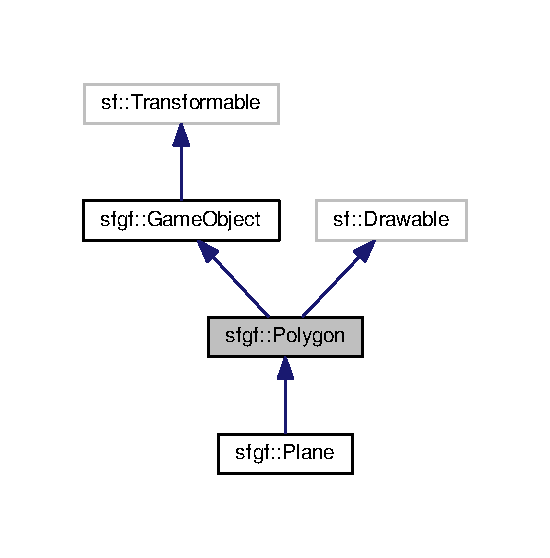
\includegraphics[width=264pt]{classsfgf_1_1Polygon__inherit__graph}
\end{center}
\end{figure}
\subsection*{Public Member Functions}
\begin{DoxyCompactItemize}
\item 
{\bfseries Polygon} (size\+\_\+t size)\hypertarget{classsfgf_1_1Polygon_ac0e3dc7fc8690145aa007fcfed22ba8c}{}\label{classsfgf_1_1Polygon_ac0e3dc7fc8690145aa007fcfed22ba8c}

\item 
void {\bfseries set\+Texture} (const sf\+::\+Texture \&tex, const std\+::vector$<$ sf\+::\+Vector2f $>$ \&tex\+Corrds)\hypertarget{classsfgf_1_1Polygon_abd78111e7f26e4750c67cf29ac56687f}{}\label{classsfgf_1_1Polygon_abd78111e7f26e4750c67cf29ac56687f}

\item 
void {\bfseries set\+Color} (sf\+::\+Color c)\hypertarget{classsfgf_1_1Polygon_a8386919ff578dbdafcfce0802f9b4ee9}{}\label{classsfgf_1_1Polygon_a8386919ff578dbdafcfce0802f9b4ee9}

\item 
void {\bfseries set\+Vertices} (const std\+::vector$<$ sf\+::\+Vector2f $>$ \&vertices)\hypertarget{classsfgf_1_1Polygon_ac2fd09fef44ed0af81a47b773a7a4de9}{}\label{classsfgf_1_1Polygon_ac2fd09fef44ed0af81a47b773a7a4de9}

\item 
const std\+::vector$<$ sf\+::\+Vertex $>$ \& {\bfseries get\+Vertices} () const \hypertarget{classsfgf_1_1Polygon_a7bee1deaa314b19f446651b556dec69c}{}\label{classsfgf_1_1Polygon_a7bee1deaa314b19f446651b556dec69c}

\item 
void {\bfseries set\+Sample\+Collider} (const \hyperlink{classsfgf_1_1Collider}{Collider} \&c)\hypertarget{classsfgf_1_1Polygon_aa44ecf16c2fa708766d94552aaceff8e}{}\label{classsfgf_1_1Polygon_aa44ecf16c2fa708766d94552aaceff8e}

\item 
const \hyperlink{classsfgf_1_1Collider}{Collider} \& {\bfseries get\+Sample\+Collider} () const \hypertarget{classsfgf_1_1Polygon_a20c269377502a72558c55d2cb8530189}{}\label{classsfgf_1_1Polygon_a20c269377502a72558c55d2cb8530189}

\item 
const \hyperlink{classsfgf_1_1Collider}{Collider} \& {\bfseries get\+Transformed\+Collider} () const \hypertarget{classsfgf_1_1Polygon_ab8edf97fc02407d2ea5548e99a8110f8}{}\label{classsfgf_1_1Polygon_ab8edf97fc02407d2ea5548e99a8110f8}

\item 
\hyperlink{classsfgf_1_1Collider}{Collider} {\bfseries get\+Default\+Sample\+Collider} () const \hypertarget{classsfgf_1_1Polygon_a4c414f102f071f4bb249660998bbef85}{}\label{classsfgf_1_1Polygon_a4c414f102f071f4bb249660998bbef85}

\item 
void {\bfseries update\+Collider} ()\hypertarget{classsfgf_1_1Polygon_a46e0ea175d0cde1b1ef252299c83c58b}{}\label{classsfgf_1_1Polygon_a46e0ea175d0cde1b1ef252299c83c58b}

\item 
virtual void {\bfseries update} (sf\+::\+Time)\hypertarget{classsfgf_1_1Polygon_a175546b9b45787e783684d28f0281eea}{}\label{classsfgf_1_1Polygon_a175546b9b45787e783684d28f0281eea}

\item 
bool {\bfseries contains} (sf\+::\+Vector2f point) const \hypertarget{classsfgf_1_1Polygon_a6f02e5633538e728a35e27346517e6e1}{}\label{classsfgf_1_1Polygon_a6f02e5633538e728a35e27346517e6e1}

\item 
bool {\bfseries intersects} (\hyperlink{classsfgf_1_1Polygon}{Polygon} \&poly) const \hypertarget{classsfgf_1_1Polygon_ade7f35a67281ac16b89db0e9291a9953}{}\label{classsfgf_1_1Polygon_ade7f35a67281ac16b89db0e9291a9953}

\item 
bool {\bfseries collides} (\hyperlink{classsfgf_1_1Polygon}{Polygon} \&poly) const \hypertarget{classsfgf_1_1Polygon_adb1b2f7577c70c89c671b569a57a13ca}{}\label{classsfgf_1_1Polygon_adb1b2f7577c70c89c671b569a57a13ca}

\item 
sf\+::\+Float\+Rect {\bfseries get\+Global\+Bounds} () const \hypertarget{classsfgf_1_1Polygon_a412b42bdff02c0c757993e099b5834af}{}\label{classsfgf_1_1Polygon_a412b42bdff02c0c757993e099b5834af}

\end{DoxyCompactItemize}


The documentation for this class was generated from the following file\+:\begin{DoxyCompactItemize}
\item 
S\+F\+G\+F/Polygon.\+hpp\end{DoxyCompactItemize}

\chapter{File Documentation}
\hypertarget{Collider_8hpp}{}\section{S\+F\+G\+F/\+Collider.hpp File Reference}
\label{Collider_8hpp}\index{S\+F\+G\+F/\+Collider.\+hpp@{S\+F\+G\+F/\+Collider.\+hpp}}


Collider class implementation.  


{\ttfamily \#include $<$S\+F\+M\+L/\+Graphics/\+Transform.\+hpp$>$}\\*
{\ttfamily \#include $<$S\+F\+M\+L/\+System/\+Vector2.\+hpp$>$}\\*
{\ttfamily \#include $<$iostream$>$}\\*
{\ttfamily \#include $<$vector$>$}\\*
Include dependency graph for Collider.\+hpp\+:\nopagebreak
\begin{figure}[H]
\begin{center}
\leavevmode
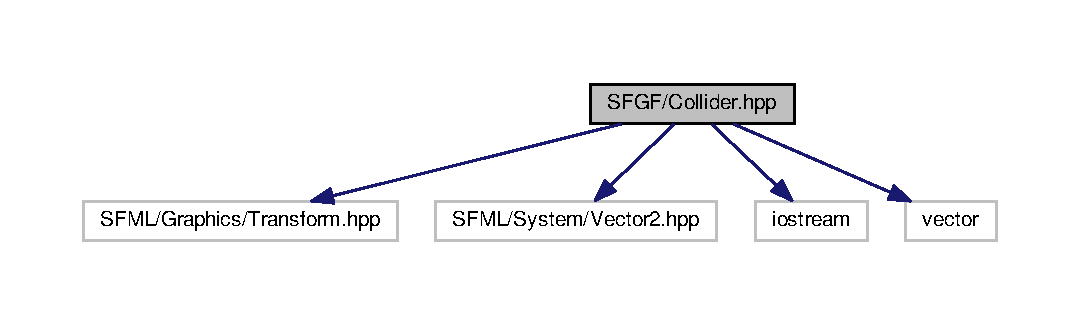
\includegraphics[width=350pt]{Collider_8hpp__incl}
\end{center}
\end{figure}
This graph shows which files directly or indirectly include this file\+:\nopagebreak
\begin{figure}[H]
\begin{center}
\leavevmode
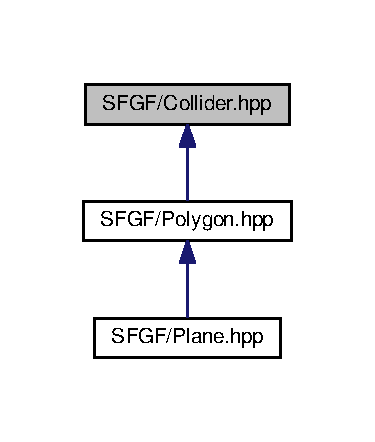
\includegraphics[width=180pt]{Collider_8hpp__dep__incl}
\end{center}
\end{figure}
\subsection*{Classes}
\begin{DoxyCompactItemize}
\item 
class \hyperlink{classsfgf_1_1Collider}{sfgf\+::\+Collider}
\begin{DoxyCompactList}\small\item\em Handles collisions. \end{DoxyCompactList}\end{DoxyCompactItemize}
\subsection*{Namespaces}
\begin{DoxyCompactItemize}
\item 
 \hyperlink{namespacesfgf}{sfgf}
\begin{DoxyCompactList}\small\item\em Contains all S\+F\+GF classes. \end{DoxyCompactList}\end{DoxyCompactItemize}


\subsection{Detailed Description}
Collider class implementation. 


%--- End generated contents ---

% Index
\backmatter
\newpage
\phantomsection
\clearemptydoublepage
\addcontentsline{toc}{chapter}{Index}
\printindex

\end{document}
